\section*{Exercice 129 -- Géométrie -- EPAS}
\setcounter{exo}{0}
% Pole JC TD 4 Sup


On s’intéresse à une Échelle Pivotante Automatique à commande Séquentielle (voir vidéo sur site internet).
Ce système, conçu et commercialisé par la société CAMIVA, est monté sur le châssis d’un camion de pompiers et permet de
déplacer une plate-forme, pouvant recevoir deux personnes et un brancard (charge maxi 270 kg), le plus rapidement
possible et en toute sécurité.

\begin{figure}[H]
\centering
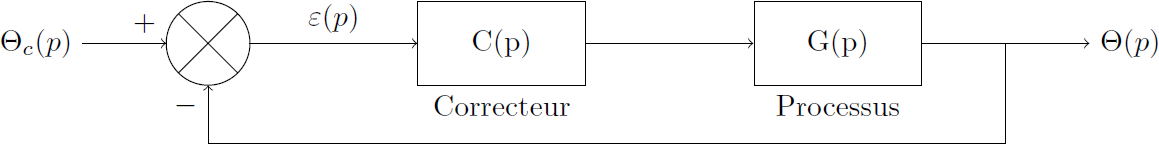
\includegraphics[width=\linewidth]{994_01}
\end{figure}

\begin{figure}[H]
\centering
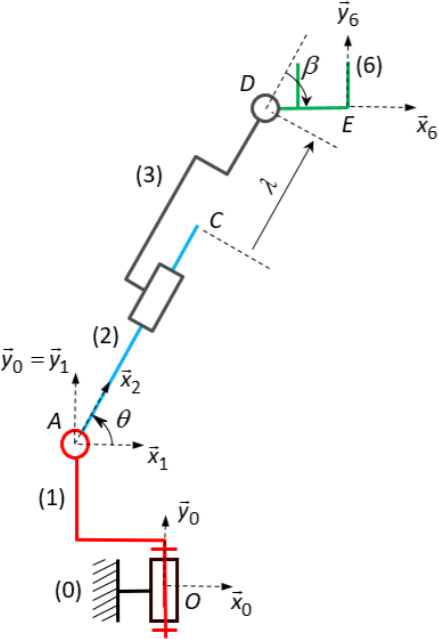
\includegraphics[width=\linewidth]{994_02}
\end{figure}



Le système est représenté, dans la situation particulière $\alpha= 0$, sous forme de schéma cinématique ci-contre .
Ce système est constitué de quatre solides, listés ci-dessous avec leur repère associé :
\begin{itemize}
\item châssis 0, $\rep{0}=\repere{0}{x_0}{y_0}{z_0}$;
\item tourelle 1, $\rep{1}=\repere{A}{x_1}{y_1}{z_1}$ tel que $\vect{y_1}=\vect{y_0}$;
\item berceau 2, $\rep{2}=\repere{A}{x_2}{y_2}{z_2}$ tel que $\vect{z_2}=\vect{z_1}$;
\item échelle 3, $\rep{3}=\repere{D}{x_3}{y_3}{z_3}$ tel que $\mathcal{B}_3=\mathcal{B}_2$;
\item plate-forme 6, $\rep{6}=\repere{E}{x_6}{y_6}{z_6}$ tel que $\vect{z_6}=\vect{z_2}$.
\end{itemize}

On donne les paramètres de mouvement :
$\alpha = \angl{x_0}{x_1}$, $\theta= \angl{x_1}{x_2}$, $\beta = \angl{x_2}{x_6}$, $\vect{CD}= \lambda \vect{x_2}$.

On donne les dimensions caractéristiques : $\vect{OA}=a\vect{x_1} + b\vect{y_1}$, $\vect{AC} = c\vect{x_2}$, $\vect{DE}=e\vect{x_6}$.

L’étude se fait pendant la phase de dressage. Pendant cette phase, la tourelle 1 est fixe par rapport au châssis 0 ( $\alpha$ = cte) et le berceau 2 s’incline de plus en plus alors que l’échelle 3 se déploie. On suppose que le châssis 0 est ancré sur le sol
parfaitement horizontal grâce aux bras de stabilisation.

On donne ci-dessous un extrait du cahier des charges : 
\begin{itemize}
\item exigence 1 : pendant la phase de dressage, la plate-forme 6 doit rester en permanence horizontale afin d’assurer la
sécurité des personnes qui sont embarquées. 
\item exigence 2 : lors d’une intervention, le point $E$ à l’extrémité de la plate-forme 6 doit se déplacer verticalement le long de la façade d’un immeuble (L= cte et $y$ variable au cours du temps).
\end{itemize}

\begin{obj}
Déterminer la loi de commande en position de chacune des chaînes d’énergie-puissance afin de
respecter les exigences du cahier des charges.
\end{obj}

\subparagraph{}
\textit{Sur le schéma cinématique, repasser chaque solide d’une couleur différente.}
\ifprof
\begin{corrige}
\end{corrige}
\else
\fi

\subparagraph{}
\textit{Réaliser le graphe des liaisons. Préciser le paramètre de mouvement associé à chaque liaison. Préciser les
éventuelles égalités de base.}
\ifprof
\begin{corrige}
\end{corrige}
\else
\fi

\subparagraph{}
\textit{Réaliser les figures de changement de base illustrant les paramètres de mouvement angulaires.}
\ifprof
\begin{corrige}
\end{corrige}
\else
\fi

\subparagraph{}
\textit{Préciser en le justifiant, le mouvement de 6/1, afin de respecter l’exigence Ex1 du cahier des charges. Que peut-on dire de la base $\mathcal{B}_6 = \base{x_6}{y_6}{z_6}$ ? Donner la relation entre $\beta$ et $\gamma$ afin de garantir ce mouvement ?}
\ifprof
\begin{corrige}
\end{corrige}
\else
\fi

\subparagraph{}
\textit{ Donner, en fonction des paramètres de mouvements et des dimensions caractéristiques du mécanisme,
l’expression du vecteur position $\vect{AE}$ du point $E$ dans le repère 1.}
\ifprof
\begin{corrige}
\end{corrige}
\else
\fi

\subparagraph{}
\textit{Donner, en fonction de $L$ et $y$ , une autre expression de ce vecteur lorsque l’exigence Ex2 est respectée.}
\ifprof
\begin{corrige}
\end{corrige}
\else
\fi

\subparagraph{}
\textit{En déduire deux relations mathématiques, traduisant l’exigence Ex2 du cahier des charges, qui lient les
paramètres de mouvement, les dimensions caractéristiques, L et y.
}
\ifprof
\begin{corrige}
\end{corrige}
\else
\fi

\subparagraph{}
\textit{ Donner alors les lois de commande en position $\lambda= f (y)$ puis $\theta = f(y)$. Conclure.}
\ifprof
\begin{corrige}
\end{corrige}
\else
\fi
